\documentclass{article}
% ------------------------------------------------------------------------------
\usepackage{amsmath, amsthm, amssymb, amsfonts}
\usepackage{thmtools}
\usepackage{graphicx}
\usepackage{setspace}
\usepackage{geometry}
\usepackage{float}
\usepackage{hyperref}
\usepackage[utf8]{inputenc}
\usepackage[english]{babel}
\usepackage{framed}
\usepackage[dvipsnames]{xcolor}
\usepackage{tcolorbox}
% ------------------------------------------------------------------------------
% Import with ```% Import with ```% Import with ```\input{utilities\new-commands}```
\newcommand{\HRule}[1]{\rule{\linewidth}{#1}}

\newcommand{\OpenDyslexic}[1]{
    {
        \defaultfontfeatures{Mapping=tex-text,Scale=MatchLowercase}
        \setmainfont{OpenDyslexic}
        \fontsize{24}{26}\selectfont\setstretch{0.5}
        #1
    }
}```
\newcommand{\HRule}[1]{\rule{\linewidth}{#1}}

\newcommand{\OpenDyslexic}[1]{
    {
        \defaultfontfeatures{Mapping=tex-text,Scale=MatchLowercase}
        \setmainfont{OpenDyslexic}
        \fontsize{24}{26}\selectfont\setstretch{0.5}
        #1
    }
}```
\newcommand{\HRule}[1]{\rule{\linewidth}{#1}}

\newcommand{\OpenDyslexic}[1]{
    {
        \defaultfontfeatures{Mapping=tex-text,Scale=MatchLowercase}
        \setmainfont{OpenDyslexic}
        \fontsize{24}{26}\selectfont\setstretch{0.5}
        #1
    }
}
% Import with ```% Import with ```% Import with ```\input{utilities\new-colors}```
\colorlet{LightGray}{White!90!Periwinkle}
\colorlet{LightOrange}{Orange!15}
\colorlet{LightGreen}{Green!15}
\definecolor{creme}{RGB}{255, 253, 208}```
\colorlet{LightGray}{White!90!Periwinkle}
\colorlet{LightOrange}{Orange!15}
\colorlet{LightGreen}{Green!15}
\definecolor{creme}{RGB}{255, 253, 208}```
\colorlet{LightGray}{White!90!Periwinkle}
\colorlet{LightOrange}{Orange!15}
\colorlet{LightGreen}{Green!15}
\definecolor{creme}{RGB}{255, 253, 208}
% ------------------------------------------------------------------------------
\declaretheoremstyle[name=Theorem,]{thmsty}
\declaretheorem[style=thmsty,numberwithin=section]{theorem}
\tcolorboxenvironment{theorem}{colback=LightGray}
% ------------------------------------------------------------------------------
\declaretheoremstyle[name=Proposition,]{prosty}
\declaretheorem[style=prosty,numberlike=theorem]{proposition}
\tcolorboxenvironment{proposition}{colback=LightOrange}
% ------------------------------------------------------------------------------
\declaretheoremstyle[name=Principle,]{prcpsty}
\declaretheorem[style=prcpsty,numberlike=theorem]{principle}
\tcolorboxenvironment{principle}{colback=LightGreen}
% ------------------------------------------------------------------------------
\setstretch{1.2}
\geometry{
    textheight=9in,
    textwidth=5.5in,
    top=1in,
    headheight=12pt,
    headsep=25pt,
    footskip=30pt}
% ------------------------------------------------------------------------------
\begin{document}
% ------------------------------------------------------------------------------
% Cover Page and ToC
% ------------------------------------------------------------------------------
    \title{ 
        \normalsize 
        \textsc{} \\
        [2.0cm]
        \HRule{1.5pt} \\
        \LARGE \textbf{
            \uppercase{
             Educational sciences}
        \HRule{2.0pt} \\ 
        [0.6cm] 
        \LARGE{
            Opdracht naam} 
        \vspace*{
            10\baselineskip}}}
    \date{}
    \author{
        \textbf{Tygo van den Hurk} \textit{(1705709)}\textbf{, \& Rik Janssen} 
        \textit{(???????)} \\ 
        \\
        20 September 2023}
    \maketitle
    \newpage
    % --------------------------------------------------------------------------
    % Table of Contents
    % --------------------------------------------------------------------------
    \tableofcontents
    \newpage
    % --------------------------------------------------------------------------
    \section{Examples}
    \begin{theorem}
        This is a theorem.
    \end{theorem}
    \begin{proposition}
        This is a proposition.
    \end{proposition}
    \begin{principle}
        This is a principle.
    \end{principle}
    \subsection{Pictures}
    \begin{figure}[htbp]
        \center
        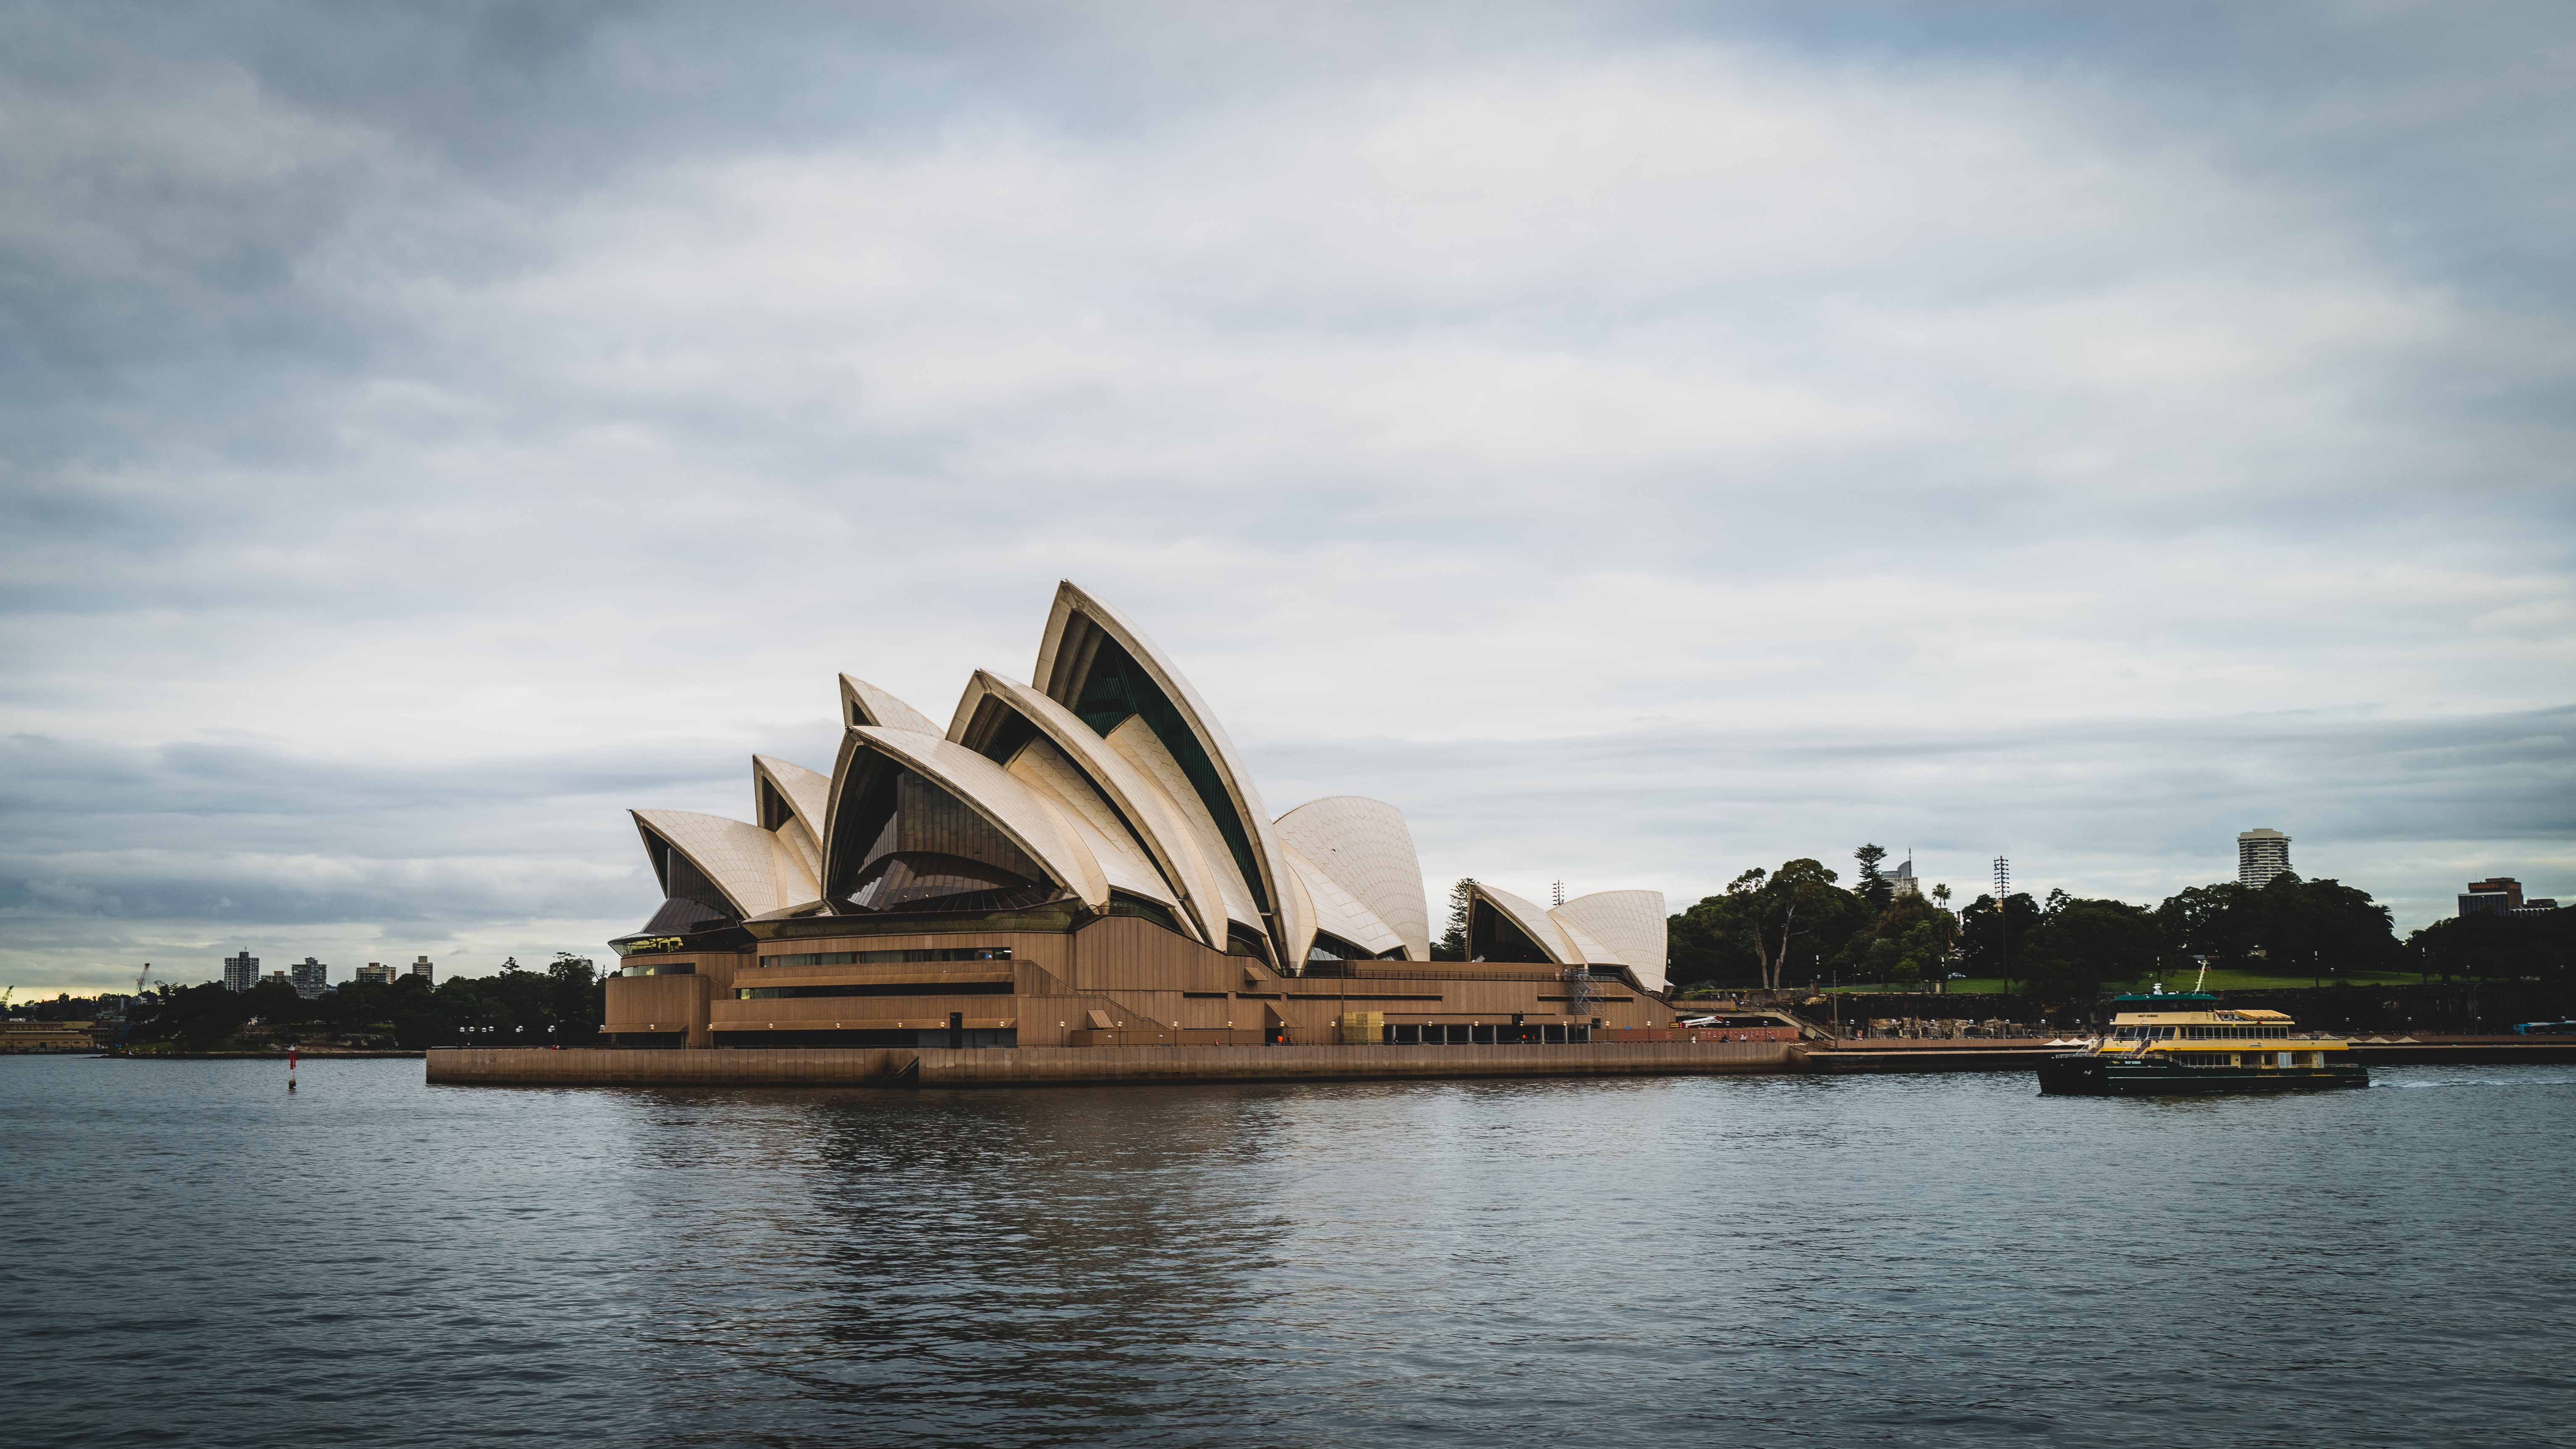
\includegraphics[scale=0.06]{images/photo.jpg}
        \caption{Sydney, NSW}
    \end{figure}
    \subsection{Citation}
    This is a citation\cite{Eg}.
    \newpage
    % ------------------------------------------------------------------------------
    % Reference and Cited Works
    % ------------------------------------------------------------------------------
    \bibliographystyle{IEEEtran}
    \bibliography{References.bib}
    % ------------------------------------------------------------------------------
\end{document}
